\documentclass[12pt]{article}
\usepackage{geometry}
\geometry{a4paper, margin=1in}
\usepackage{amsmath}
\usepackage{amssymb}
\usepackage[utf8]{vietnam}
\usepackage{hyperref}
\usepackage{graphicx}
\usepackage{setspace}
\usepackage{tocloft}
\usepackage{enumitem}
\usepackage{listings}
\usepackage{xcolor}
\usepackage{tabularx}
\usepackage{amsmath}
\usepackage{fancyhdr}
\lstset{ %
    language=SQL,                % Chọn ngôn ngữ
    basicstyle=\ttfamily\footnotesize, % Font cho đoạn mã
    keywordstyle=\color{blue},   % Màu cho từ khóa
    commentstyle=\color{gray},   % Màu cho chú thích
    stringstyle=\color{red},     % Màu cho chuỗi ký tự
    numberstyle=\tiny\color{gray}, % Kiểu đánh số dòng
    stepnumber=1,                % Bước đánh số dòng
    numbersep=5pt,               % Khoảng cách từ mã đến số dòng
    showspaces=false,            % Không hiển thị khoảng trắng
    showstringspaces=false,      % Không hiển thị khoảng trắng trong chuỗi
    breaklines=true,             % Tự động xuống dòng
    breakatwhitespace=true,      % Xuống dòng tại khoảng trắng
    frame=single,                % Khung bao quanh đoạn mã
    tabsize=4                    % Kích thước tab
}

\usepackage{background}
\usepackage{background}
\backgroundsetup{contents=
\includegraphics{hustlogo.png}, scale = 0.45, angle = 0, opacity=0.25}

\definecolor{udc}{rgb}{0.58,0.0.01,0.04} 

\renewcommand{\headrulewidth}{0pt}
\renewcommand\UrlFont{\color{blue}\rmfamily}
% set page geometry
\geometry{a4paper, total={140mm,250mm}, left=20mm, right=20mm, top=14mm, bottom=30mm}

\title{Database\\Quản lý thư viện}
\author{
\\ {Lê Hải Yến 20225780}
\\ {Nguyễn Ngân Hà 20225713}
\\ {Nguyễn Kim Ngọc 20225655}
}

\newcommand{\mails}{
\\ {yen.lh225780@sis.hust.edu.vn}
\\ {ha.nn225713@sis.hust.edu.vn}
\\ {ngoc.nk225655@sis.hust.edu.vn}
}

\newcommand{\class}{147778 - IT3290}
\newcommand{\lecturer}{{Vũ Tuyết Trinh}
\\trinh.vutuyet@hust.edu.vn
}

\date{\today}
\makeatletter{}

\usepackage{biblatex}
\addbibresource{citations.bib}

\begin{document}\backgroundsetup{contents = 
\includegraphics{soictlogo.png}, scale = 0.5, vshift = 5cm, angle = 50, opacity = 0.05} \raggedright
%%%%%%%%%%%%%%%%%%%%%%%%%%%%%%%%%%%%%%%%%%%%%%%%%%%%%%%%%%%%%%%%%%%%%%%%%%%%%%%%%%%%%%%%%%%%%%%%%%%%%%%%%%%%%%%%%%%%%%%%%%%%%%%%%%
\NoBgThispage
\thispagestyle{empty}

	\newcommand{\HRule}{\rule{\linewidth}{0.3mm}} 
	\begin{center}
	    
	
  \MakeUppercase{\large Hanoi University of Science and Technology} \\[0.5cm]
   
  {\LARGE School of Information and Communication Technology} \\[0.5cm]
		{
\includegraphics[width=0.25\textwidth]{hustlogo.png} \par}\vspace{0.5cm}
	\textsc	{\MakeUppercase{\Large BÁO CÁO PROJECT THỰC HÀNH CƠ SỞ DỮ LIỆU}\\[0.75cm]}
	
	\textsc	{\MakeUppercase{\large Thực hành cơ sở dữ liệu\\\normalsize (IT3290)}\\[0.5cm]}
	
	\HRule\\[0.4cm]

	{\huge\bfseries \@title}\\[0.4cm]
	\HRule\\[1.5cm]
		\begin{center}
			\large
			\textit{Nhóm 9}\\
		\end{center}
	
	\begin{minipage}{0.4\textwidth}
		\begin{flushleft}
			\large
			\textit{Thành viên}\\
			\@author
		\end{flushleft}
	\end{minipage}
	~
	\begin{minipage}{0.4\textwidth}
		\begin{flushright}
			\large
			\textit{Email}\\
	\mails 
		\end{flushright}
	\end{minipage}
\vfill\vfill
\vspace{0.3cm}
        \begin{minipage}{0.4\textwidth}
		\begin{center}
			\large
			\textit{Lớp}\\
			\class\\
			\textit{Giảng viên}\\
			\lecturer\\
		\end{center}
	\end{minipage}
\vfill\vfill
\vspace{0.3cm}
    \vfill\vfill
    \normalsize{\today}
    \\[0.3cm]

    
    \vfill
  \end{center}  
\newpage
\begin{center}
   \large \textbf{Báo cáo\\}
   \normalsize \textbf{Database quản lý thư viện\\}
   \small
   Lớp: 147778\\
   Giảng viên: Vũ Tuyết Trinh\\
    
\end{center}
\tableofcontents % Tạo mục lục
\clearpage % Chuyển sang trang mới

\noindent \textbf{Ý tưởng khởi đầu}:
Trong bối cảnh công nghệ ngày càng phát triển, việc quản lý và tối ưu hóa hoạt động của các thư viện trở nên cần thiết hơn bao giờ hết. Để đáp ứng nhu cầu ngày càng cao của bạn đọc và tăng cường hiệu quả quản lý tài nguyên, một hệ thống cơ sở dữ liệu quản lý thư viện hiện đại và thông minh là giải pháp tối ưu. Hệ thống này không chỉ giúp các quản trị viên dễ dàng theo dõi, quản lý sách và tài liệu mà còn tạo điều kiện cho người dùng tìm kiếm, mượn và trả sách một cách thuận tiện và nhanh chóng. Tất cả các thông tin liên quan đến sách, bạn đọc, và các hoạt động mượn trả đều được lưu trữ và cập nhật tự động, đảm bảo tính minh bạch và chính xác, đồng thời hỗ trợ các quyết định quản lý hiệu quả hơn.

\section{Mô tả bài toán}

\subsection{Mô tả sơ bộ}
\begin{itemize}[leftmargin=1.5cm]
    \item \textbf{Nền tảng cho phép độc giả (người đọc) có thể mượn sách, tìm kiếm tài liệu, và theo dõi tình trạng mượn trả sách:} Hệ thống cho phép người dùng tra cứu danh mục sách, kiểm tra tình trạng sẵn có của sách, và thực hiện các thao tác mượn trả sách trực tuyến. Độc giả có thể đăng nhập vào tài khoản cá nhân để quản lý lịch sử mượn trả sách và nhận thông báo về hạn trả sách.
    \item \textbf{Cho phép nhân viên quản lý tài nguyên thư viện một cách hiệu quả:} Hệ thống hỗ trợ các nhân viên thư viện trong việc quản lý và cập nhật danh mục sách, theo dõi tình trạng mượn trả sách của độc giả, và xử lý các yêu cầu từ độc giả. Ngoài ra, nhân viên có thể sử dụng hệ thống để lập báo cáo về tình trạng tài nguyên, thống kê mượn trả sách, và theo dõi các hoạt động khác trong thư viện.
\end{itemize}

\subsection{Quản lý các hoạt động}
Quản lý hoạt động trong hệ thống quản lý cơ sở dữ liệu thư viện bao gồm việc theo dõi và điều phối tất cả các hoạt động hàng ngày của thư viện, đảm bảo rằng mọi quy trình diễn ra một cách trôi chảy và hiệu quả.
\subsubsection*{Người Đọc (Độc Giả) Có Thể:}

\begin{itemize}
    \item \textbf{Đăng ký tài khoản}: Đăng ký tài khoản mới với thông tin cá nhân như tên, địa chỉ, số điện thoại, email, ngày đăng ký.
    \item \textbf{Tìm kiếm sách}: Tìm kiếm sách theo tiêu đề, tác giả, thể loại, nhà xuất bản, năm xuất bản, v.v.
    \item \textbf{Mượn sách}: Đăng ký mượn sách qua hệ thống, xem thông tin sách và kiểm tra tính khả dụng của sách.
    \item \textbf{Trả sách}: Trả sách qua hệ thống, ghi nhận ngày trả và tình trạng sách khi trả.
    \item \textbf{Nhận thông báo}: Nhận thông báo về sách sắp đến hạn trả, sách quá hạn, các sự kiện sắp diễn ra qua email hoặc SMS.
    \item \textbf{Xem lịch sử mượn/trả sách}: Xem lịch sử các sách đã mượn và trả, bao gồm ngày mượn, ngày trả, và tình trạng sách.
\end{itemize}

\subsubsection*{Nhân Viên Có Thể:}

\begin{itemize}
    \item \textbf{Quản lý người đọc}: Thêm mới, chỉnh sửa, hoặc xóa thông tin người đọc.
    \item \textbf{Quản lý sách}: 
    \begin{itemize}
        \item Thêm mới, chỉnh sửa, hoặc xóa thông tin sách.
        \item Kiểm kê số lượng sách, cập nhật tình trạng sách (sách mất, sách hư hỏng).
    \end{itemize}
    \item \textbf{Xử lý giao dịch mượn/trả sách}: 
    \begin{itemize}
        \item Ghi nhận và quản lý các giao dịch mượn sách và trả sách của người đọc.
        \item Tính toán và ghi nhận phí phạt khi trả sách muộn.
    \end{itemize}
    \item \textbf{Quản lý tài liệu số}: 
    \begin{itemize}
        \item Số hóa tài liệu, thêm mới và quản lý kho tài liệu số.
        \item Cung cấp quyền truy cập và quản lý việc sử dụng tài liệu số bởi người đọc.
    \end{itemize}
    \item \textbf{Báo cáo và thống kê}: 
    \begin{itemize}
        \item Tạo các báo cáo và thống kê về sách mượn/trả, hoạt động của người đọc, tài chính, và các sự kiện.
    \end{itemize}
\end{itemize}

\section{Thiết kế cơ sở dữ liệu}
\subsection{Mô hình thực thể liên kết}
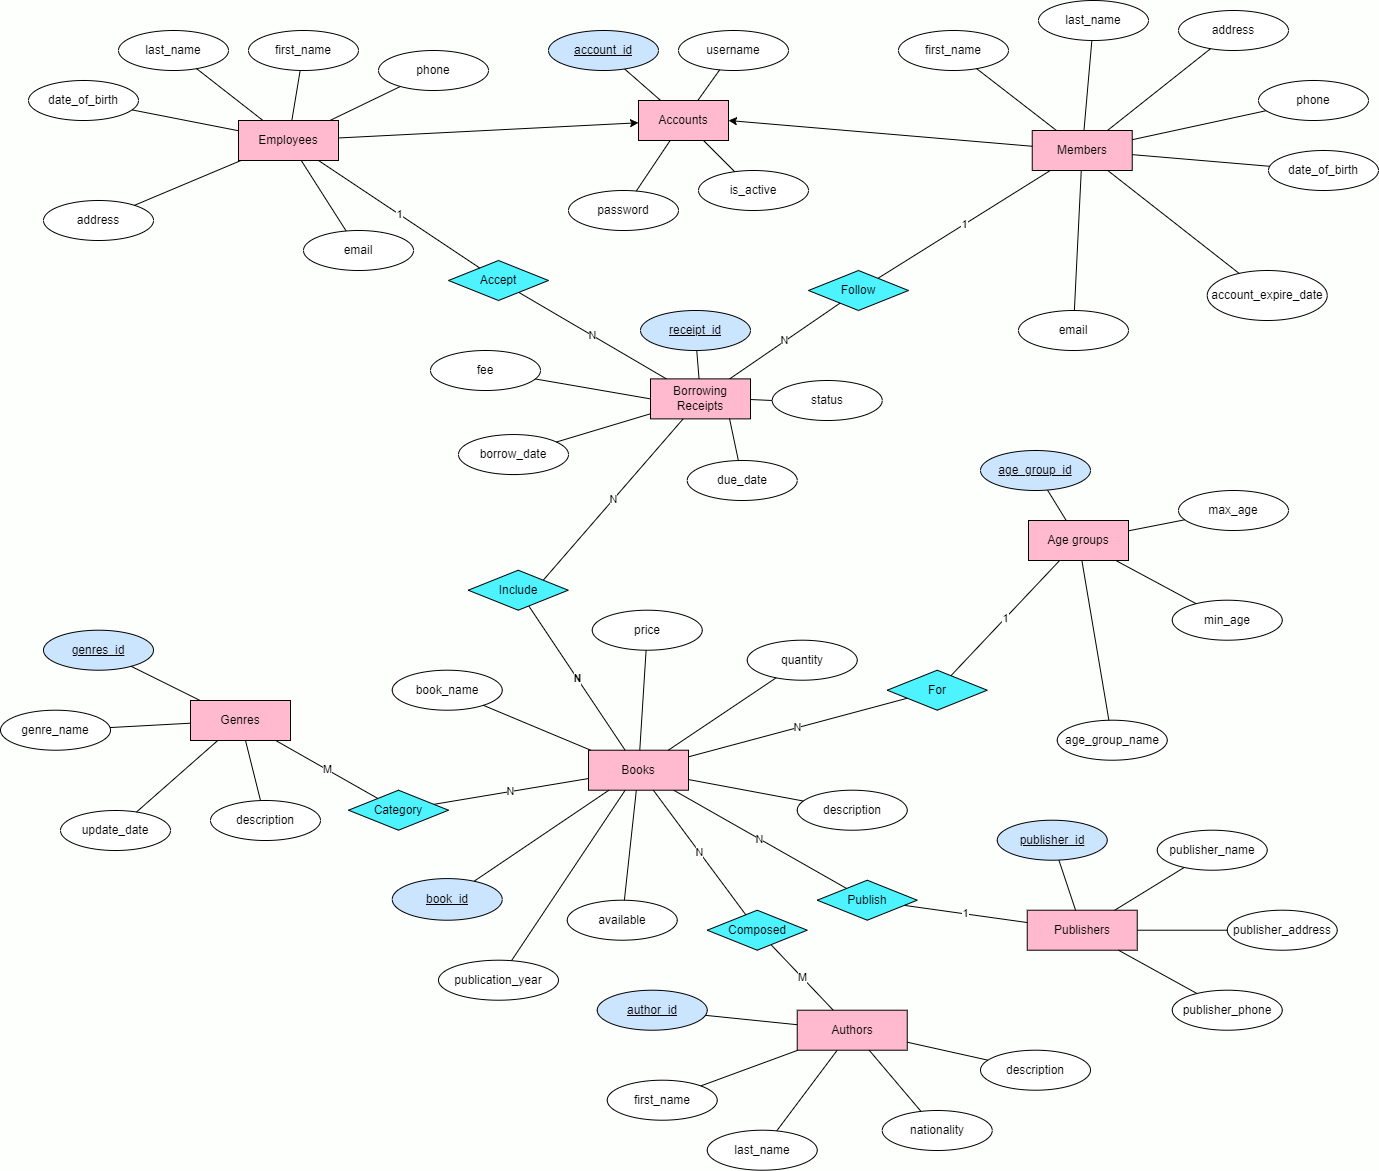
\includegraphics[width=1\textwidth]{SDTTLK.png}
\subsection{Chi tiết các bảng}
\begin{itemize}[leftmargin=1.5cm]
    \item Thông tin về tài khoản (Accounts) bao gồm: Mã định danh tài khoản (account\_id), tên đăng nhập (username), mật khẩu (password\_id), trạng thái hoạt động tài khoản (is\_active).
    \item Thông tin về nhân viên (Employees) bao gồm: Tên (first\_name), họ (last\_name), ngày sinh (date\_of\_birth), số điện thoại (phone), địa chỉ (address), email (email).
    \item Thông tin về khách hàng (Members) bao gồm: Tên (first\_name), họ (last\_name), ngày sinh (date\_of\_birth), số điện thoại (phone), địa chỉ (address), email (email), ngày hết hạn thành viên (expire\_date).
    \item Thông tin về thể loại sách (Genres) bao gồm: Mã định danh thể loại sách (genre\_id), tên thể loại sách (genre\_name).
    \item Thông tin về tác giả (Authors) bao gồm: Mã định danh tác giả (author\_id), tên (first\_name), họ (last\_name), quốc tịch (nationality).
    \item Thông tin về nhóm tuổi (Age\_groups) bao gồm: Mã định danh nhóm tuổi (age\_group\_id), tên nhóm tuổi (age\_group\_name), tuổi tối thiểu (min\_age), tuổi tối đa (max\_age).
    \item Thông tin về sách (Books) bao gồm: Mã định danh sách (book\_id), tên sách (book\_name), mã định danh nhóm tuổi (age\_group\_id), mã định danh nhà xuất bản (publisher\_id), năm xuất bản (publication\_year), số lượng sách hiện có (available), tổng số lượng sách (quantity), giá sách (price).
    \item Thông tin về phiếu mượn sách (Borrowing\_Receipts) bao gồm: Mã định danh phiếu mượn (receipt\_id), mã định danh tài khoản nhân viên (employee\_account\_id), mã định danh tài khoản khách hàng (member\_account\_id), mã định danh sách (book\_id), mã định danh phí phạt (fee\_id), ngày mượn (borrow\_date), ngày dự kiến trả (due\_date), ngày trả thực tế (return\_date), trạng thái phiếu mượn (status), phí phạt (fee).
\end{itemize}
\subsection{Mô hình quan hệ}
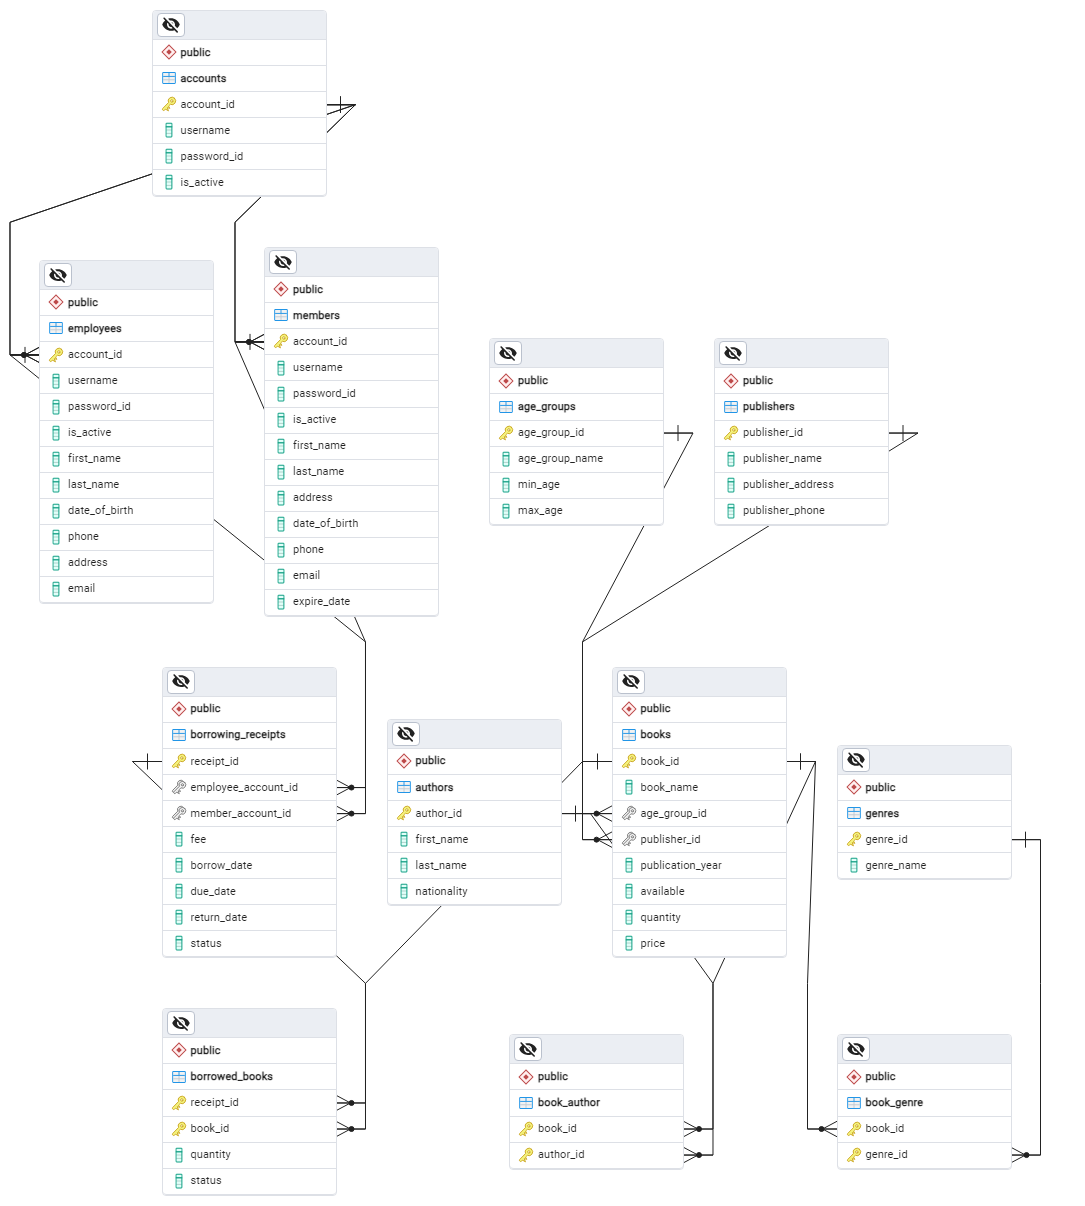
\includegraphics[width=0.85\textwidth]{Untitled.png}
\subsection{Quan hệ giữa các bảng}
\begin{itemize}
    \item Quan hệ giữa Accounts và Employees là quan hệ một-một (1-1).
    \item Quan hệ giữa Accounts và Members là quan hệ một-một (1-1).  
    \item Quan hệ giữa Books và Authors là quan hệ nhiều-nhiều (N-N), thông qua bảng trung gian Book\_Authors.
    \item Quan hệ giữa Books và Genres là quan hệ một-nhiều (1-N).
    \item Quan hệ giữa Books và Publishers là quan hệ một-nhiều (1-N).
    \item Quan hệ giữa Books và Age\_groups là quan hệ nhiều-một (N-1).
    \item Quan hệ giữa Borrowing\_Receipts và Books là quan hệ nhiều-nhiều (N-N), thông qua bảng trung gian Borrowed\_Books.
    \item Quan hệ giữa Borrowing\_Receipts và Employees là quan hệ nhiều-một (N-1).
    \item Quan hệ giữa Borrowing\_Receipts và Members là quan hệ nhiều-một (N-1).
\end{itemize}
\section{Các chức năng thực hiện}
\subsection{Chức năng sử dụng Query}
\begin{enumerate}
    \item Trả về top 10 đầu sách thỏa mãn có số lượng người mượn nhiều nhất trong 1 tháng kể từ thời gian gần nhất:
    \begin{enumerate}
        \item Truy vấn:
        \begin{lstlisting}
WITH RecentMonthBorrowers AS (
    SELECT DISTINCT br.receipt_id
    FROM Borrowing_Receipts br
    WHERE br.borrow_date < DATE_TRUNC('month', CURRENT_DATE)
    AND br.borrow_date >= DATE_TRUNC('month', CURRENT_DATE - INTERVAL '1 month')
),
BooksBorrowed AS (
    SELECT bb.book_id, COUNT(DISTINCT br.receipt_id) AS borrower_count
    FROM Borrowed_Books bb
    INNER JOIN Borrowing_Receipts br ON bb.receipt_id = br.receipt_id
    WHERE br.receipt_id IN (SELECT receipt_id FROM RecentMonthBorrowers)
    GROUP BY bb.book_id
)
SELECT b.book_name, bb.borrower_count
FROM Books b
INNER JOIN BooksBorrowed bb ON b.book_id = bb.book_id
ORDER BY bb.borrower_count DESC
LIMIT 10

        \end{lstlisting}
        \item Kết quả:
        
        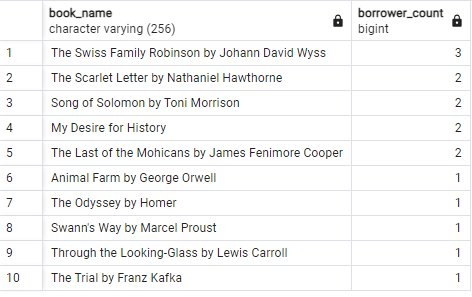
\includegraphics[width= 0.5\textwidth]{Screenshot 2024-06-22 014242.png}
    \end{enumerate}
    \item Tìm ra top 3 người mượn sách có số lượt mượn cao nhất trong mỗi nhóm tuổi (dựa trên các khoảng tuổi được xác định trước), trong 3 tháng trước:
    \begin{enumerate}
        \item Truy vấn:
        \begin{lstlisting}
WITH MemberAgeGroup AS (
    SELECT
        m.account_id,
        m.first_name,
        m.last_name,
        m.date_of_birth,
        ag.age_group_id,
        ag.age_group_name,
        EXTRACT(YEAR FROM AGE(CURRENT_DATE, m.date_of_birth)) AS age
    FROM
        Members m
        JOIN Age_groups ag ON (
            EXTRACT(YEAR FROM AGE(CURRENT_DATE, m.date_of_birth)) BETWEEN ag.min_age AND ag.max_age
        )
),
MemberBorrowCount AS (
    SELECT
        m.account_id,
        m.first_name,
        m.last_name,
        mag.age_group_id,
        mag.age_group_name,
        COUNT(br.receipt_id) AS borrow_count
    FROM
        Borrowing_Receipts br
        JOIN Members m ON br.member_account_id = m.account_id
        JOIN MemberAgeGroup mag ON m.account_id = mag.account_id
    WHERE
        br.borrow_date >= date_trunc('month', CURRENT_DATE) - INTERVAL '3 months'
        AND br.borrow_date < date_trunc('month', CURRENT_DATE)
    GROUP BY
        m.account_id,
        m.first_name,
        m.last_name,
        mag.age_group_id,
        mag.age_group_name
),
RankedMembers AS (
    SELECT
        mbc.*,
        ROW_NUMBER() OVER (PARTITION BY mbc.age_group_id ORDER BY mbc.borrow_count DESC) AS rank
    FROM
        MemberBorrowCount mbc
)
SELECT
    age_group_id,
    age_group_name,
    account_id,
    first_name,
    last_name,
    borrow_count
FROM
    RankedMembers
WHERE
    rank <= 3
ORDER BY
    age_group_id,
    rank;
        \end{lstlisting}
        \item Kết quả:
        
        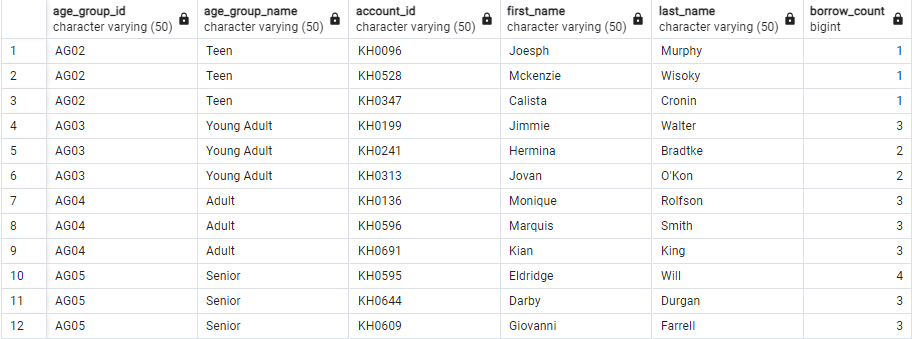
\includegraphics[width= 0.8\textwidth]{Screenshot 2024-06-22 015329.png}
    \end{enumerate}
    \item Đưa ra nhóm tuổi có số lượng người nhiều nhất:
    \begin{enumerate}
        \item Truy vấn:
        \begin{lstlisting}
WITH MemberAges AS (
    SELECT 
		m.account_id, 
		EXTRACT(YEAR FROM AGE(CURRENT_DATE, m.date_of_birth)) AS age
    FROM Members m
),
AgeGroupCounts AS (
    SELECT 
		ag.age_group_name,
		COUNT(ma.account_id) AS member_count
    FROM MemberAges ma
    JOIN Age_groups ag ON ma.age BETWEEN ag.min_age AND ag.max_age
    GROUP BY ag.age_group_name
)
SELECT age_group_name, member_count
FROM AgeGroupCounts
ORDER BY member_count DESC
LIMIT 1;
        \end{lstlisting}
        \item Kết quả:
        
        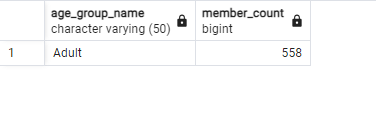
\includegraphics[width= 0.5\textwidth]{Screenshot 2024-06-22 020149.png}
    \end{enumerate}
    \item Tính số phần trăm đơn mượn sách trả đúng hạn:
    \begin{enumerate}
        \item Truy vấn:
        \begin{lstlisting}
SELECT 
    ROUND((COUNT(CASE WHEN return_date <= due_date THEN 1 END)::numeric / COUNT(*) * 100), 2) AS percent_on_time
FROM 
    Borrowing_Receipts
WHERE 
    return_date IS NOT NULL;
        \end{lstlisting}
        \item Kết quả:
        
        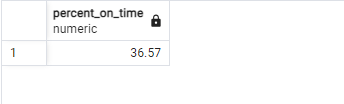
\includegraphics[width= 0.4\textwidth]{Screenshot 2024-06-22 021925.png}
    \end{enumerate}
    \item Tính số phần trăm của các member mà tài khoản còn hoạt động trong từng nhóm tuổi:
    \begin{enumerate}
        \item Truy vấn:
        \begin{lstlisting}
WITH TotalMembers AS (
    SELECT
        AG.age_group_id,
        AG.age_group_name,
        COUNT(M.date_of_birth) AS total_members
    FROM
        Age_groups AG
    LEFT JOIN
        Members M ON EXTRACT(YEAR FROM AGE(M.date_of_birth)) BETWEEN AG.min_age AND AG.max_age
    GROUP BY
        AG.age_group_id, AG.age_group_name
),
ActiveMembers AS (
    SELECT
        AG.age_group_id,
        AG.age_group_name,
        COUNT(M.date_of_birth) AS active_members
    FROM
        Age_groups AG
    LEFT JOIN
        Members M ON EXTRACT(YEAR FROM AGE(M.date_of_birth)) BETWEEN AG.min_age AND AG.max_age
    WHERE
        M.is_active = true
    GROUP BY
        AG.age_group_id, AG.age_group_name
)
SELECT
    TM.age_group_id,
    TM.age_group_name,
    TM.total_members,
    COALESCE(AM.active_members, 0) AS active_members,
    CASE
        WHEN TM.total_members > 0 THEN (AM.active_members::numeric / TM.total_members::numeric) * 100
        ELSE 0
    END AS active_percentage
FROM
    TotalMembers TM
LEFT JOIN
    ActiveMembers AM ON TM.age_group_id = AM.age_group_id
ORDER BY
    TM.age_group_id;
        \end{lstlisting}
        \item Kết quả:
        
        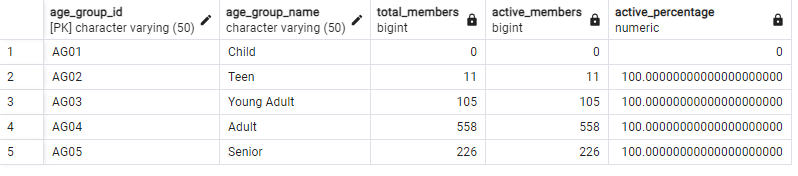
\includegraphics[width= 0.8\textwidth]{Screenshot 2024-06-22 022220.png}
    \end{enumerate}
    \item Đưa ra 5 đầu sách mà lứa tuổi già (senior) ưa thích nhất trong 1 năm vừa qua:
    \begin{enumerate}
    \item Truy vấn:
    \begin{lstlisting}
WITH SeniorMembers AS (
    SELECT m.account_id
    FROM Members m
    JOIN Age_groups ag ON EXTRACT(YEAR FROM AGE(CURRENT_DATE, m.date_of_birth)) BETWEEN ag.min_age AND ag.max_age
),
RecentSeniorBorrowings AS (
    SELECT bb.book_id, COUNT(DISTINCT bb.receipt_id) AS borrow_count
    FROM SeniorMembers sm
    JOIN Borrowing_Receipts br ON sm.account_id = br.member_account_id
    JOIN Borrowed_Books bb ON br.receipt_id = bb.receipt_id
    WHERE br.borrow_date >= DATE_TRUNC('year', CURRENT_DATE) - INTERVAL '1 year'
    GROUP BY bb.book_id
)
SELECT b.book_name, rsb.borrow_count
FROM RecentSeniorBorrowings rsb
JOIN Books b ON rsb.book_id = b.book_id
ORDER BY rsb.borrow_count DESC
LIMIT 5;
    \end{lstlisting}
    \item Kết quả:
        
        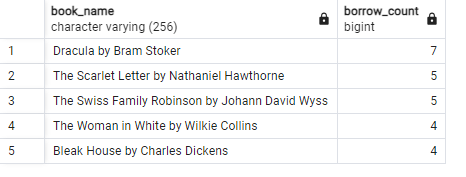
\includegraphics[width= 0.6\textwidth]{Screenshot 2024-06-22 144118.png}
    \end{enumerate}

\item Thêm tác giả cho sách:
    \begin{enumerate}
        \item Truy vấn:
        \begin{lstlisting}
INSERT INTO Book_Author (book_id, author_id)
VALUES ('BK0016', 'AT0001'); 
        \end{lstlisting}
        \item Kết quả:\\
        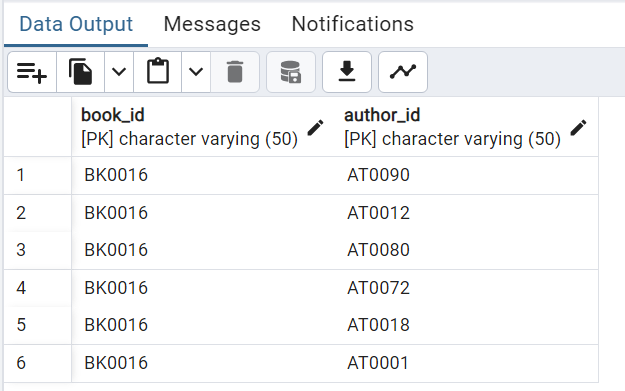
\includegraphics[width= 0.6\textwidth]{query1.png}
    \end{enumerate}
    
 \item In ra danh sách sách mượn trong 1 đơn:
    \begin{enumerate}
        \item Truy vấn:
        \begin{lstlisting}
SELECT
    b.book_id,
    b.book_name,
    bb.quantity,
    b.price
FROM
    Borrowed_Books bb
    JOIN Books b ON bb.book_id = b.book_id
WHERE
    bb.receipt_id = 'BR0003'; 
        \end{lstlisting}
        \item Kết quả:\\
        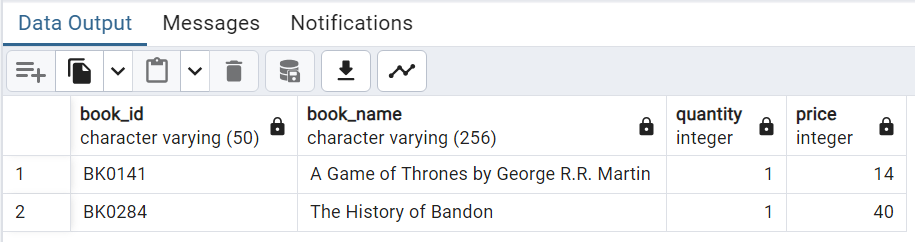
\includegraphics[width= 0.6\textwidth]{query2.png}
    \end{enumerate}   

 \item In ra danh sách tên các sách cho độ tuổi child:
    \begin{enumerate}
        \item Truy vấn:
        \begin{lstlisting}
    SELECT
    b.book_id,
    b.book_name,
    b.publisher_id,
    b.publication_year,
    b.available,
    b.quantity,
    b.price
FROM
    Books b
    JOIN Age_groups ag ON b.age_group_id = ag.age_group_id
WHERE
    ag.age_group_name = 'Child';
        \end{lstlisting}
        \item Kết quả:\\
        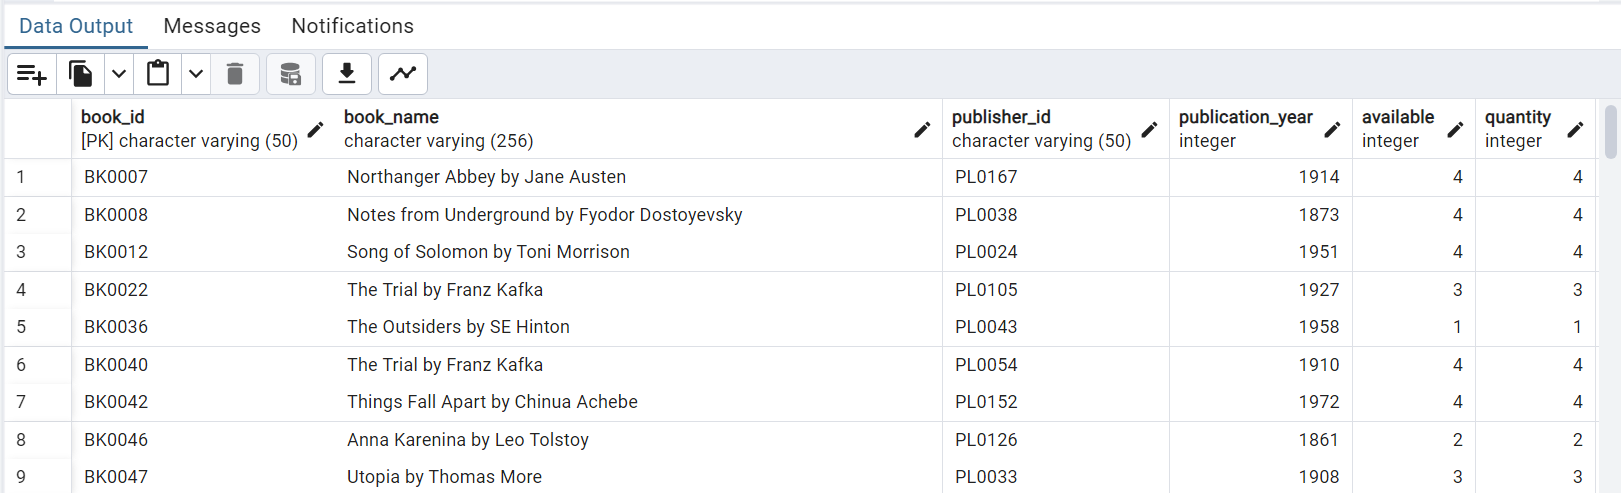
\includegraphics[width= 0.8\textwidth]{query3.png}
    \end{enumerate} 

    \item Cập nhật giá sách:
    \begin{enumerate}
        \item Truy vấn:
        \begin{lstlisting}
UPDATE Books SET price = 100
WHERE book_id = 'BK0001';
        \end{lstlisting}
        \item Kết quả:\\
        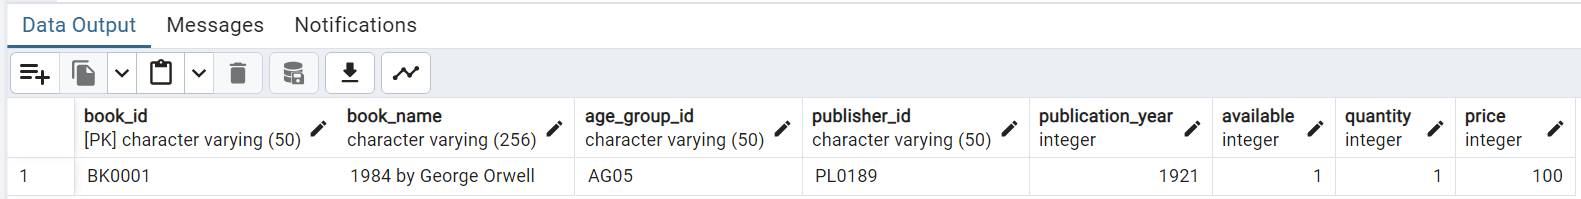
\includegraphics[width= 0.8\textwidth]{query4.png}
    \end{enumerate}



\end{enumerate}
\subsection{Chức năng sử dụng Trigger}
\begin{enumerate}
    \item Cập nhật lại số available khi có sách được mượn, trả và xử lý trường hợp mượn quá số lượng available:
    \begin{enumerate}
        \item Code:
    \begin{lstlisting}       
DECLARE
    v_total_borrowed INTEGER;
BEGIN
    IF TG_OP = 'INSERT' AND NEW.status = 'Borrowing' THEN
        SELECT SUM(quantity) INTO v_total_borrowed
        FROM Borrowed_Books
        WHERE receipt_id = NEW.receipt_id;

        IF v_total_borrowed > (SELECT available FROM Books WHERE book_id = NEW.book_id) THEN
            UPDATE Borrowing_Receipts
            SET status = 'Canceled'
            WHERE receipt_id = NEW.receipt_id;
        ELSE
            UPDATE Books
            SET available = available - NEW.quantity
            WHERE book_id = NEW.book_id;
        END IF;
    END IF;

    IF TG_OP = 'UPDATE' AND NEW.status = 'Returned' AND OLD.status = 'Borrowing' THEN
        UPDATE Books
        SET available = available + NEW.quantity
        WHERE book_id = NEW.book_id;
    END IF;

    RETURN NEW;
END;
    \end{lstlisting}
    \item Giải thích:
    
    Khi người dùng mượn sách và thêm vào bảng Borrowed\_Books cùng với số lượng sách, trigger sẽ kiểm tra xem tổng số lượng sách đã mượn có vượt quá số lượng có sẵn của sách đó hay không. Nếu vượt quá, đơn mượn tương ứng sẽ được đưa về trạng thái Canceled. Ngược lại, số lượng sách có sẵn sẽ được cập nhật bằng cách trừ đi số lượng sách đã mượn.
    Khi người dùng trả sách, trigger sẽ cập nhật trạng thái của sách đó thành Returned. Đồng thời, số lượng sách có sẵn sẽ được cập nhật bằng cách cộng thêm số lượng sách đã trả vào số lượng có sẵn hiện tại.
    \item  Demo:
    \begin{itemize}
    \item Ta có sách với book\_id là "BK0028" với available = 5
        \begin{lstlisting}
SELECT * FROM public.books
	WHERE book_id = 'BK0028'
ORDER BY book_id ASC 
    \end{lstlisting}
    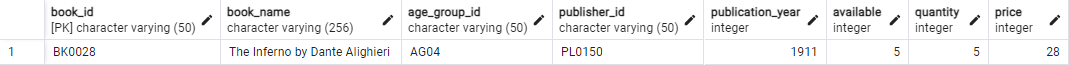
\includegraphics[width=1\linewidth]{Screenshot 2024-06-23 020340.png}
    \item Khi mượn 3 cuốn sách đấy thì available bằng 2
    \begin{lstlisting}
INSERT INTO public.borrowed_books(
	receipt_id, book_id, quantity, status)
	VALUES ('BR0206','BK0028' ,3 ,'Borrowing' );

    \end{lstlisting}
    
 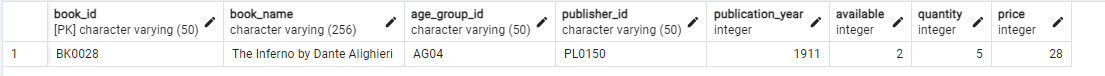
\includegraphics[width=1\linewidth]{6.png}
    \item Và khi trả lại sách ( cập nhật trạng thái sách là Returned ) thì available bằng 5
    \begin{lstlisting}
UPDATE public.borrowed_books
	SET status= 'Returned'
	WHERE receipt_id= 'BR0206' AND book_id = 'BK0028';
    \end{lstlisting}
    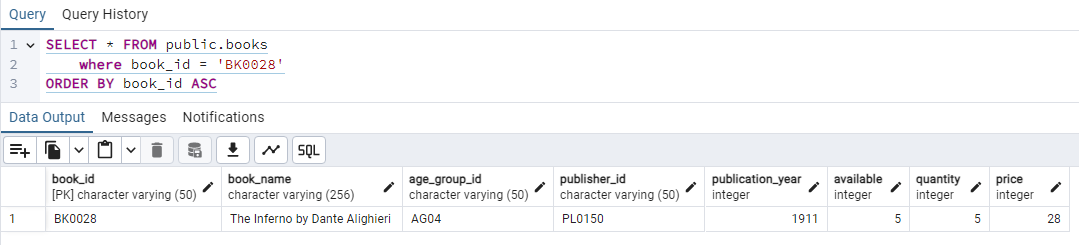
\includegraphics[width=1\linewidth]{image1.png}
    \item Nếu mượn 6 cuốn ( vượt quá available là 5 ) thì giữ nguyên available và đưa trạng thái của đơn mượn về Canceled
    \begin{lstlisting}
INSERT INTO borrowed_books(
	receipt_id, book_id, quantity, status)
	VALUES ('BR0308','BK0028' ,6 ,'Borrowing' );
    \end{lstlisting}
    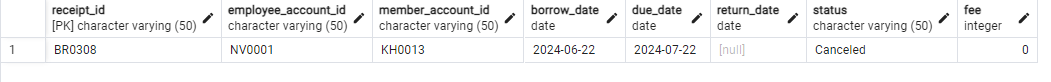
\includegraphics[width=1\linewidth]{5.png}

     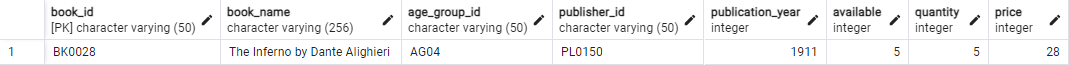
\includegraphics[width=1\linewidth]{Screenshot 2024-06-23 020340.png}
    \end{itemize}
    \end{enumerate}
    \item Cập nhật is\_active nếu tài khoản member còn hạn:
    \begin{enumerate}
        \item Code:
    \begin{lstlisting}
BEGIN
    IF NEW.expire_date > CURRENT_DATE THEN
        UPDATE Accounts
        SET is_active = TRUE
        WHERE account_id = NEW.account_id;
    END IF;
    
    RETURN NEW;
END;
    \end{lstlisting}
    \item Giải thích:

    Khi ta thêm 1 tài khoản người dùng vào với hạn tài khoản lớn hơn thời gian thực thì is\_active của accounts sẽ nhận giá trị là TRUE
    \item Demo:
    Ta insert người dùng với expired\_date là \'2025-06-23\' thì ta được is\_active của account đó là TRUE
    \begin{lstlisting}
INSERT INTO public.members(
	account_id, username, password_id, is_active, first_name, last_name, address, date_of_birth, phone, email, expire_date)
	VALUES ('KH9999','TUMROYAL' ,'TUM123',FALSE ,'NGoc' ,'KIM' ,'VietNam' ,'25-07-2004' ,'1203120312' ,'ndasdns@gmail.com' ,'23-12-2024' ); 
    \end{lstlisting}
    \begin{lstlisting}
SELECT is_active FROM public.members
WHERE account_id = 'KH9999'
    \end{lstlisting}
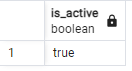
\includegraphics[width=0.2\linewidth]{7.png}
    \end{enumerate}
    
    \item Kiểm tra tổng sách giới hạn được mượn (có thể mượn nhiều nhất là 10 cuốn):
    \begin{enumerate}
        \item Code:
    \begin{lstlisting} 
DECLARE
    total_books_member INT;
BEGIN
    SELECT SUM(bb.quantity)
    INTO total_books_member
    FROM Borrowed_Books bb
    JOIN Borrowing_Receipts br ON bb.receipt_id = br.receipt_id
    WHERE br.member_account_id = (SELECT member_account_id FROM Borrowing_Receipts WHERE receipt_id = NEW.receipt_id)
    AND bb.status = 'Borrowing';

    IF total_books_member + NEW.quantity > 10 THEN 
        RAISE EXCEPTION 'The total number of borrowed books for the member exceeds the limit of 10. Current total: %', total_books_member;
    END IF;

    RETURN NEW;
END;
    \end{lstlisting}
    \item Giải thích: 
    
    Quy định rằng mỗi người chỉ được mượn tối đa 10 cuốn sách. Khi thực hiện mượn sách, nếu tổng số sách đang được mượn và số sách sắp được mượn vượt quá 10, hệ thống sẽ thông báo lỗi và không cho phép tạo đơn mượn mới (không thể thực hiện thêm vào).
    \item Kết quả:
    \begin{itemize}
        \item Ta có người dùng với id là "KH0023" đang mượn số sách là 9 cuốn
        \begin{lstlisting}
SELECT br.member_account_id,
       COUNT(bb.book_id) AS total_borrowed_books,
       SUM(bb.quantity) AS total_quantity_borrowed
FROM Borrowing_Receipts br
JOIN Borrowed_Books bb ON br.receipt_id = bb.receipt_id
WHERE bb.status = 'Borrowing' AND member_account_id = 'KH0023'
GROUP BY br.member_account_id;
        \end{lstlisting}
        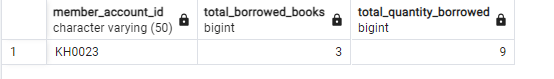
\includegraphics[width=1\linewidth]{Screenshot 2024-06-23 032337.png}
        \item tạo đơn mượn thêm 2 cuốn sách nữa cho người dùng này thì:
        \begin{lstlisting}
INSERT INTO borrowed_books(
	receipt_id, book_id, quantity, status)
	VALUES ('BR0311','BK0042' ,2 ,'Borrowing' );
        \end{lstlisting}
        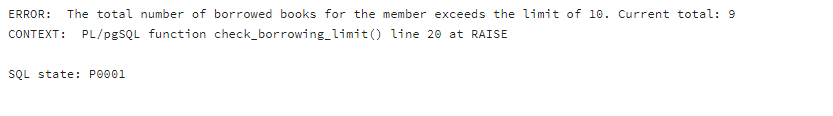
\includegraphics[width=1.1\linewidth]{10.png}
    \end{itemize}
    
    
    
    \end{enumerate}
    \item Cập nhật trạng thái và ngày trả của đơn mượn:
    
    \begin{enumerate}
        \item Code:
    \begin{lstlisting}
DECLARE
    total_returned_books INTEGER;
    total_borrowed_books INTEGER;
BEGIN
    SELECT COUNT(DISTINCT book_id) INTO total_borrowed_books
    FROM borrowed_books
    WHERE receipt_id = NEW.receipt_id;

    SELECT COUNT(DISTINCT book_id) INTO total_returned_books
    FROM borrowed_books
    WHERE receipt_id = NEW.receipt_id AND (status = 'Returned' OR status = 'Lost');

    IF total_returned_books = total_borrowed_books THEN
        UPDATE borrowing_receipts
        SET status = 'Returned', return_date = CURRENT_DATE
        WHERE receipt_id = NEW.receipt_id;
    ELSE
        UPDATE borrowing_receipts
        SET status = 'Borrowing', return_date = NULL
        WHERE receipt_id = NEW.receipt_id;
    END IF;

    RETURN NEW;
END;
    \end{lstlisting}
    \item Giải thích:

Khi người dùng trả sách, hệ thống sẽ cập nhật trạng thái của từng cuốn sách mà người dùng đã mượn. Nếu tất cả các sách trong một đơn mượn đã được trả, hệ thống sẽ cập nhật trạng thái của đơn mượn thành "Returned" và ghi nhận thời điểm trả là thời gian hiện tại.
    \item Demo
    \begin{itemize}
        \item Ta có đơn mượn "BR0311" có 2 sách được mượn với trạng thái Borrowing
        
        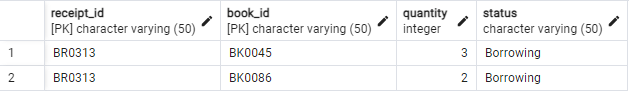
\includegraphics[width=0.8\linewidth]{Screenshot 2024-06-23 040728.png}
        \item Cập nhật trạng thái 2 sách này khi được người dùng trả
        \begin{lstlisting}
UPDATE public.borrowed_books
	SET status='Returned'
	WHERE receipt_id = 'BR0313' AND (book_id = 'BK0045' OR book_id = 'BK0086')
        \end{lstlisting}
        \item Kết quả trả về status của đơn mượn là Return
        
        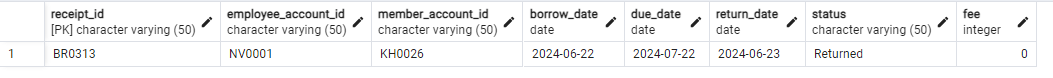
\includegraphics[width=1.1\linewidth]{12.png}
    \end{itemize}
    \end{enumerate}
    \item Cập nhật fee phải trả khi trả sách:
    \begin{enumerate}
        \item Code:
    \begin{lstlisting}
DECLARE
    days_overdue INT;
    fee_amount INT;
    total_book_price INT;
    account_ids INT;
BEGIN
    IF NEW.return_date IS NOT NULL THEN
        days_overdue := NEW.return_date - NEW.due_date;
    ELSE
        days_overdue := CURRENT_DATE - NEW.due_date;
    END IF;

    IF days_overdue > 5 AND days_overdue <= 10 THEN
        fee_amount := 10000;
    ELSIF days_overdue > 10 AND days_overdue <= 30 THEN
        fee_amount := 20000;
    ELSIF days_overdue > 30 AND days_overdue <= 60 THEN
        fee_amount := 30000;
    ELSIF days_overdue > 60 THEN
		fee_amount := 200000;
    ELSE
        fee_amount := 0;
    END IF;

    UPDATE Borrowing_Receipts
	SET fee = fee_amount
	WHERE receipt_id = NEW.receipt_id;

    RETURN NEW;
END;
    \end{lstlisting}
    \item Giải thích:

    Khi bạn trả sách muộn, hệ thống sẽ tính phí phạt dựa trên số ngày trả muộn so với ngày hẹn trả. Các mức phạt được áp dụng như sau:
    \begin{itemize}
        \item Trả sách trong vòng 6 ngày kể từ ngày hẹn trả: Không bị phạt.
        \item Trả sách từ 6 đến 10 ngày muộn: Phí phạt là 10,000 đồng.
        \item Trả sách từ 11 đến 30 ngày muộn: Phí phạt là 20,000 đồng.
        \item Trả sách từ 31 đến 60 ngày muộn: Phí phạt là 30,000 đồng.
        \item Trả sách quá 60 ngày muộn: Phí phạt là 200,000 đồng.
    \end{itemize}
    Đây là cách hệ thống tính toán và áp dụng các khoản phí phạt khi bạn trả sách quá hạn.
    \item Demo:
    \begin{itemize}
        \item Ta có 1 đơn mượn như sau:
        
        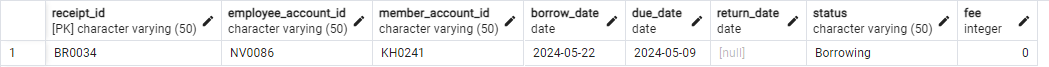
\includegraphics[width=1\linewidth]{13.png}
        \item Khi ta cập nhật ngày trả là 23-6-2024 thì fee sẽ được tính là 30000
        \begin{lstlisting}
UPDATE public.borrowing_receipts
	SET return_date= '2024-6-23'
	WHERE receipt_id = 'BR0034';
        \end{lstlisting}
        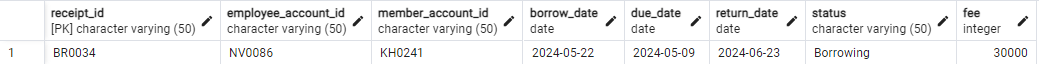
\includegraphics[width=1\linewidth]{14.png}
    \end{itemize}
    \end{enumerate}
    \item Cập nhật fee nếu có sách bị mất khi trả sách:
    
    \begin{enumerate}
        \item Code:
    
    \begin{lstlisting}
DECLARE
    lost_fee INT := 0;
    book_price INT;
    quantity_lost INT;
BEGIN
    IF NEW.status = 'Lost' THEN
        SELECT price INTO book_price
        FROM Books
        WHERE book_id = NEW.book_id;

        quantity_lost := NEW.quantity;
        lost_fee := book_price * quantity_lost;

    UPDATE Borrowing_Receipts
	SET fee = lost_fee + fee
	WHERE receipt_id = NEW.receipt_id;
    END IF;

    RETURN NEW;
END;
    \end{lstlisting}
    \item Giải thích:

    Khi có sách bị mất, người dùng phải đền bù 1 số tiền bằng giá của quyển sách. Khi đó ta cập nhật tiền đó vào phí trả sách muộn.
    \end{enumerate}
    \item Cập nhật trạng thái đơn mượn khi trả sách
    \begin{enumerate}
        \item Code:
        \begin{lstlisting}
BEGIN
    -- Check if return_date is updated and not null
    IF NEW.return_date IS NOT NULL THEN
        -- Update the status to 'Returned'
        NEW.status := 'Returned';
    END IF;
    RETURN NEW;
END;
        \end{lstlisting}
        \item Giải thích: 

        Khi người dùng trả sách, ta update ngày trả sách và trigger sẽ giúp ta update trạng thái của đơn mượn.
    \end{enumerate}
        \item Kiểm tra ngày sinh và ngày hạn tài khoản của member khi nhập vào
    \begin{enumerate}
        \item Code:
        \begin{lstlisting}
BEGIN
    IF NEW.date_of_birth > CURRENT_DATE - INTERVAL '3 years' THEN
        RAISE EXCEPTION 'Date of birth must be at least 3 years ago';
    END IF;

    IF NEW.expire_date < NEW.date_of_birth + INTERVAL '6 years' THEN
        RAISE EXCEPTION 'Expire date must be at least 6 years after date of birth';
    END IF;

    RETURN NEW;
END;
        \end{lstlisting}
        \item Giải thích: 

        Khi thêm hay cập nhật một tài khoản member thì ngày member đó phải ít nhất là 3 tuổi và ngày hạn của tài khoản phải lớn hơn ngày sinh ít nhất 6 năm nghĩa là tài khoản sẽ còn hoạt động ít nhất là 3 năm đối với mỗi một member.
        \item Kết quả:
        \begin{itemize}
        \item Khi Insert một tài khoản member mà member đó nhỏ hơn hoặc bằng 3 tuổi:
        \begin{lstlisting}
INSERT INTO members (account_id, username, password_id, is_active, first_name, last_name, address, date_of_birth, phone, email)
VALUES ('KH9998', 'john_doe', 'password123', true, 'John', 'Doe', '123 Main St', '2022-02-02', '123-456-7890', 'john.doe@example.com'); 
    \end{lstlisting}
    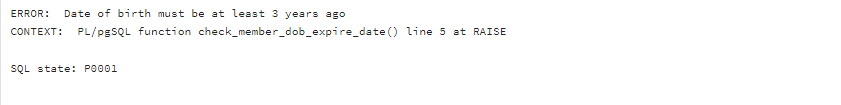
\includegraphics[width=1\linewidth]{dtb6.png}
        \item Khi Insert một tài khoản member mà hạn của tài khoản bằng ngày sinh của :
        \begin{lstlisting}
INSERT INTO members (account_id, username, password_id, is_active, first_name, last_name, address, date_of_birth, phone, email, expire_date)
VALUES ('KH9997', 'john_doe', 'password123', true, 'John', 'Doe', '123 Main St', '1999-02-02', '123-456-7890', 'john.doe@example.com', '1999-02-02'); 
    \end{lstlisting}
    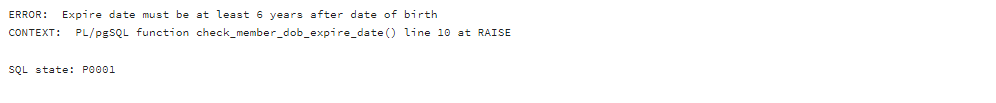
\includegraphics[width=1\linewidth]{dtb7.png}
        \end{itemize}
    \end{enumerate}
        \item Khi cập nhật thêm quantity mới cho một sách thì cũng cập nhật available mới cho sách 
    \begin{enumerate}
        \item Code:
        \begin{lstlisting}
BEGIN
    IF NEW.quantity > OLD.quantity THEN
        UPDATE public.books
        SET available = available + (NEW.quantity - OLD.quantity)
        WHERE book_id = NEW.book_id;
    ELSIF NEW.quantity < OLD.quantity THEN
        RAISE EXCEPTION 'New quantity cannot be less than the old quantity';
    END IF;

    RETURN NEW;
END;
        \end{lstlisting}
        \item Giải thích: 

        Khi cập nhật thêm số quantity cho một sách thì số lượng available cho sách đó sẽ được cộng thêm với số lượng sách đã thêm vào trong quantity. 
        \item Kết quả:
        \begin{lstlisting}
UPDATE books
SET quantity = 3
WHERE book_id = 'BK0001';

SELECT * FROM books WHERE book_id = 'BK0001'; 
    \end{lstlisting}
    \begin{itemize}
        \item Đầu tiên số lượng sách là 1:\\
        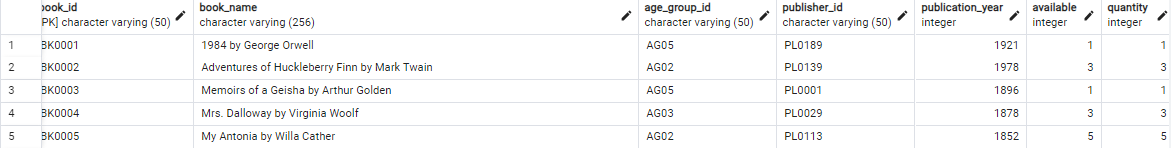
\includegraphics[width=1\linewidth]{dtb8.png}
        \item Sau khi cập nhật số lượng sách là 3 nghĩa là thêm 2 cuốn sách mới cho book\_id là 'BK0001':\\
        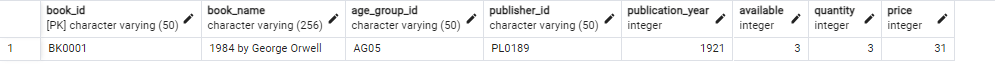
\includegraphics[width=1\linewidth]{dtb9.png}
    \end{itemize}
\end{enumerate}
\end{enumerate}
\subsection{Chức năng sử dụng Function}
\begin{enumerate}
    \item Tìm kiếm sách theo tên tác giả:
    \begin{enumerate}
        \item Code:
        
        \begin{lstlisting}
DECLARE
    v_first_name VARCHAR;
    v_last_name VARCHAR;
BEGIN
    v_first_name := split_part(Aname, ' ', 1);
    v_last_name := split_part(Aname, ' ', 2);

    RETURN QUERY
    SELECT
        b.book_id,
        b.book_name,
        CAST(CONCAT(a.first_name, ' ', a.last_name) AS VARCHAR) AS author_name,
        b.publication_year,
        b.available
    FROM
        Books b
        JOIN Book_Author ba ON b.book_id = ba.book_id
        JOIN Authors a ON ba.author_id = a.author_id
    WHERE
        a.first_name ILIKE '%' || v_first_name || '%'
        AND a.last_name ILIKE '%' || v_last_name || '%';
END;
        \end{lstlisting}

        \item Kết quả:
        
        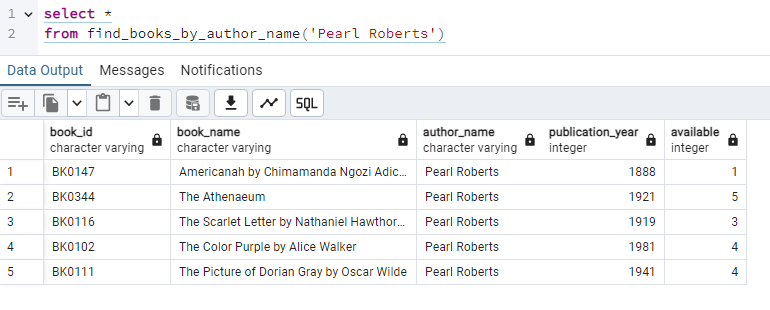
\includegraphics[width= 0.8\textwidth]{Screenshot 2024-06-22 164310.png}
    \end{enumerate}
        \item Tìm kiếm sách theo từ khóa:
    \begin{enumerate}
        \item Code:
        
        \begin{lstlisting}
BEGIN
    RETURN QUERY
    SELECT DISTINCT ON (b.book_id)
        b.book_id,
        b.book_name,
        CAST(CONCAT(a.first_name, ' ', a.last_name) AS VARCHAR) AS author_name,
        b.publication_year,
        b.available,
        g.genre_name
    FROM
        Books b
        LEFT JOIN Book_Author ba ON b.book_id = ba.book_id
        LEFT JOIN Authors a ON ba.author_id = a.author_id
        LEFT JOIN Book_Genre bg ON b.book_id = bg.book_id
        LEFT JOIN Genres g ON bg.genre_id = g.genre_id
    WHERE
        b.book_name ILIKE '%' || keyword || '%'
        OR (a.first_name ILIKE '%' || keyword || '%' AND a.last_name ILIKE '%' || keyword || '%')
        OR g.genre_name ILIKE '%' || keyword || '%';
END;
        \end{lstlisting}

        \item Kết quả:
        
        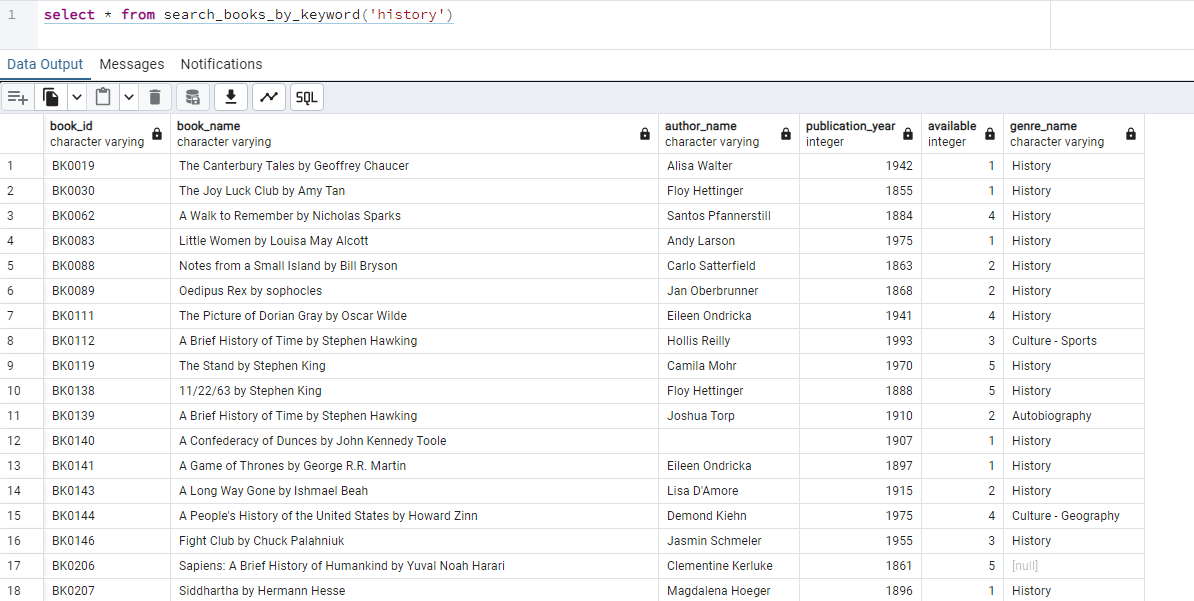
\includegraphics[width= 1\textwidth]{Screenshot 2024-06-22 170520.png}
    \end{enumerate}
    \item Hàm đưa ra độ tuổi của người đọc:
    \begin{enumerate}
        \item Code:
        
        \begin{lstlisting}
DECLARE
    age INT;
    age_group_names VARCHAR(50);
BEGIN
    SELECT EXTRACT(YEAR FROM age(current_date, birth_date)) INTO age;

    SELECT age_group_name INTO age_group_names
    FROM Age_groups
    WHERE age BETWEEN min_age AND max_age;

    RETURN age_group_names;
END;
        \end{lstlisting}

        \item Kết quả:
        
        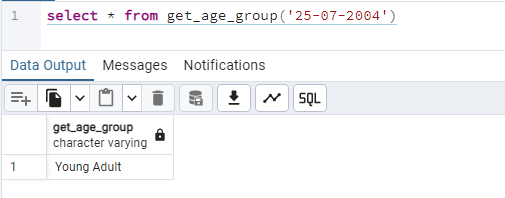
\includegraphics[width= 0.6\textwidth]{Screenshot 2024-06-22 171151.png}
    \end{enumerate}
    \item Trả về tác giả có nhiều sách nhất trong thư viện:
    \begin{enumerate}
        \item Code:
        
        \begin{lstlisting}
BEGIN
    RETURN QUERY
    SELECT
        A.author_id,
        A.first_name,
        A.last_name,
        A.nationality,
        COUNT(*) AS book_count
    FROM
        Authors A
    INNER JOIN
        Book_Author BA ON A.author_id = BA.author_id
    GROUP BY
        A.author_id, A.first_name, A.last_name, A.nationality
    ORDER BY
        book_count DESC
    LIMIT 1;
END;
        \end{lstlisting}

        \item Kết quả:
        
        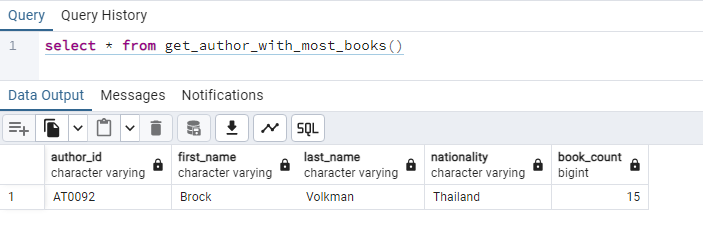
\includegraphics[width= 0.6\textwidth]{Screenshot 2024-06-22 172023.png}
    \end{enumerate}
    \item Đưa ra thống kê tổng số đơn mượn sách từng tháng trong 1 năm:
    \begin{enumerate}
        \item Code:
        
        \begin{lstlisting}
DECLARE
    month_counter INTEGER := 1;
BEGIN
    FOR month_counter IN 1..12 LOOP
        RETURN QUERY
        SELECT
            month_counter,
            COUNT(*)
        FROM
            Borrowing_Receipts BR
        WHERE
            EXTRACT(MONTH FROM BR.borrow_date) = month_counter
            AND EXTRACT(YEAR FROM BR.borrow_date) = year_input;
    END LOOP;
END;
        \end{lstlisting}

        \item Kết quả:

        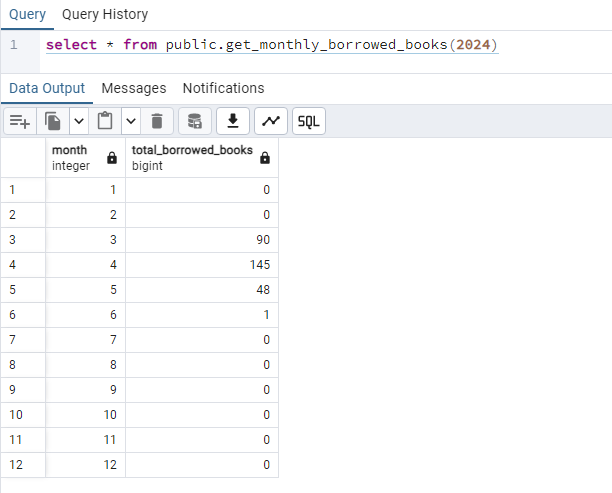
\includegraphics[width=0.8\linewidth]{Screenshot 2024-06-22 182010.png}
    \end{enumerate}

     \item Hàm trả về số lượng sách mượn của người dùng theo tháng sắp xếp giảm dần:
    \begin{enumerate}
        \item Code:
        
        \begin{lstlisting}
CREATE OR REPLACE FUNCTION get_borrowers_by_month(year_param integer, month_param integer)
RETURNS TABLE(
    member_account_id character varying(50),
    first_name character varying(50),
    last_name character varying(50),
    total_books_borrowed integer
) AS $$
BEGIN
    RETURN QUERY
    SELECT
        m.account_id AS member_account_id,
        m.first_name,
        m.last_name,
        COALESCE(SUM(bb.quantity), 0)::integer AS total_books_borrowed
    FROM
        Members m
    JOIN
        Borrowing_Receipts br ON m.account_id = br.member_account_id
    JOIN
        Borrowed_Books bb ON br.receipt_id = bb.receipt_id
    WHERE
        EXTRACT(YEAR FROM br.borrow_date) = year_param
        AND EXTRACT(MONTH FROM br.borrow_date) = month_param
    GROUP BY
        m.account_id, m.first_name, m.last_name
    ORDER BY
        total_books_borrowed DESC;
END;
$$ LANGUAGE plpgsql;
        \end{lstlisting}

        \item Kết quả:
        
        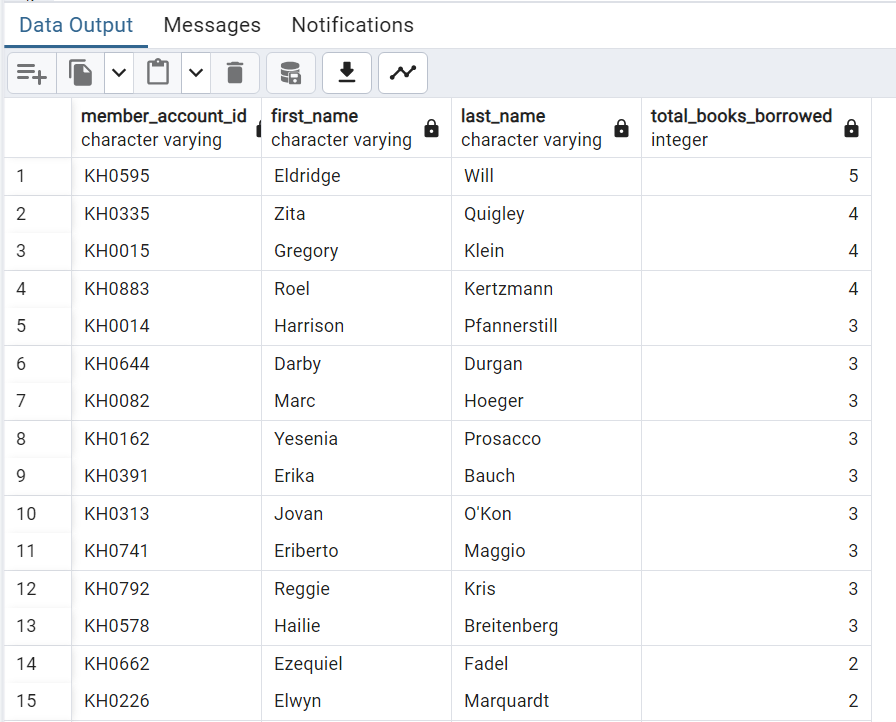
\includegraphics[width= 0.7\textwidth]{func1.png}
    \end{enumerate}

         \item Hàm trả về sách đang được mượn và số lượng:
    \begin{enumerate}
        \item Code:
        
        \begin{lstlisting}
BEGIN
    RETURN QUERY
    SELECT
        b.book_id,
        b.book_name,
        COALESCE(SUM(bb.quantity), 0)::INT AS total_borrowed_quantity
    FROM
        Books b
    JOIN
        Borrowed_Books bb ON b.book_id = bb.book_id
    JOIN
        Borrowing_Receipts br ON bb.receipt_id = br.receipt_id
    WHERE
        br.return_date IS NULL
    GROUP BY
        b.book_id, b.book_name
    ORDER BY
        total_borrowed_quantity DESC;
END;
        \end{lstlisting}

        \item Kết quả:
        
        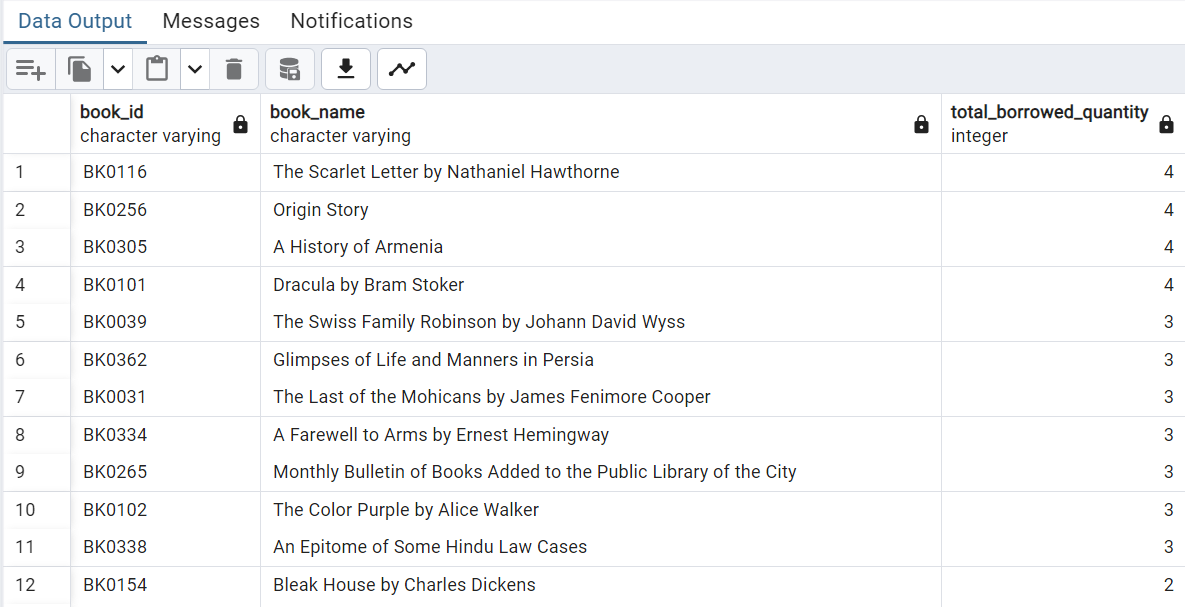
\includegraphics[width= 0.9\textwidth]{func2.png}
    \end{enumerate}
    \item Hàm trả về số sách của 1 người dùng đang mượn và hạn trả:
    \begin{enumerate}
        \item Code:
        
        \begin{lstlisting}
BEGIN
    RETURN QUERY
    SELECT
        b.book_name,
        bb.quantity,
        br.due_date
    FROM
        Borrowed_Books bb
        JOIN Books b ON bb.book_id = b.book_id
        JOIN Borrowing_Receipts br ON bb.receipt_id = br.receipt_id
    WHERE
        bb.status = 'Borrowing'
        AND br.member_account_id = p_account_id; 
END;
        \end{lstlisting}

        \item Kết quả:

        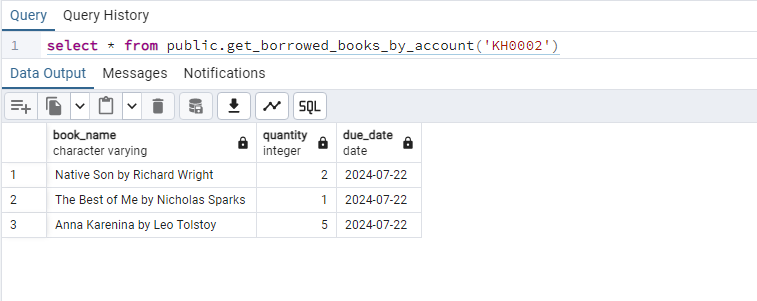
\includegraphics[width= 0.8\textwidth]{20.png}
    \end{enumerate}
\end{enumerate}
\subsection{Chức năng sử dụng Procedure}
\begin{enumerate}
    \item Xóa các tài khoản không kích hoạt
    \begin{enumerate}
        Code:
        \begin{lstlisting}
BEGIN
    DELETE FROM Members
    WHERE is_active = FALSE;
END;
        \end{lstlisting}
    \end{enumerate}
    \item Thêm sách vào thư viện
    \begin{enumerate}
        \item  Code:
        \begin{lstlisting}
DECLARE
    new_id VARCHAR;
BEGIN
    -- Generate book_id from sequence book_id_seq
    SELECT 'BK' || to_char(nextval('book_id_seq'), 'FM0000') INTO new_id;

    -- Insert new book into Books table
    INSERT INTO Books (book_id, book_name, age_group_id, publisher_id, publication_year, available, quantity, price)
    VALUES (new_id, p_book_name, p_age_group_id, p_publisher_id, p_publication_year, p_quantity, p_quantity, p_price);

    -- Print success message
    RAISE NOTICE 'Book % has been added successfully with ID %.', p_book_name, new_id;
END;
        \end{lstlisting}
        \item Kết quả:

    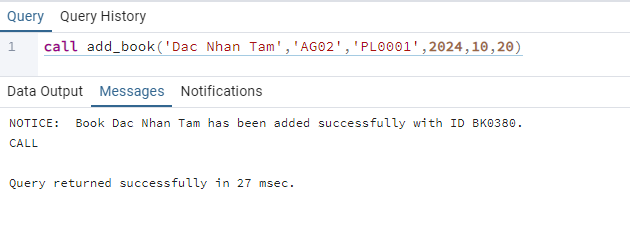
\includegraphics[width=0.8\linewidth]{image.png}
    \end{enumerate}
    \item Thêm thể loại sách:
    \begin{enumerate}
        \item  Code:
        \begin{lstlisting}
DECLARE
    new_id VARCHAR;
BEGIN
    SELECT 'G' || to_char(nextval('genre_id_seq'), 'FM0000') INTO new_id;

    INSERT INTO Genres (genre_id, genre_name)
    VALUES (new_id, p_genre_name);

    RAISE NOTICE 'Genre % has been successfully added with ID %.', p_genre_name, new_id;
END;
        \end{lstlisting}
        \item Kết quả:

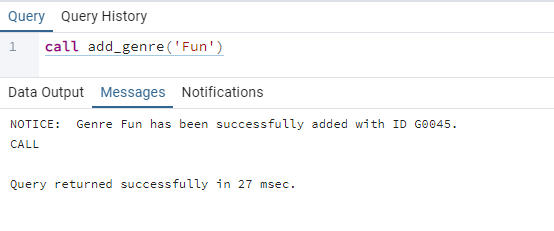
\includegraphics[width=0.8\linewidth]{1.png}
    \end{enumerate}
    \item Thêm tác giả:
    \begin{enumerate}
        \item  Code:
        \begin{lstlisting}
DECLARE
    v_author_id VARCHAR;
BEGIN
    -- Generate author_id in the format ATxxxx
    SELECT 'AT' || to_char(nextval('author_id_seq'), 'FM0000') INTO v_author_id;

    -- Insert into Authors table
    INSERT INTO Authors (author_id, first_name, last_name, nationality)
    VALUES (v_author_id, p_first_name, p_last_name, p_nationality);

    -- Print a notice message upon successful insertion
    RAISE NOTICE 'Author added successfully with author_id: %', v_author_id;
END;
        \end{lstlisting}
        \item Kết quả:

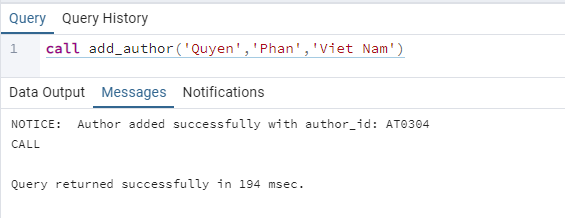
\includegraphics[width=0.8\linewidth]{Screenshot 2024-06-22 182405.png}
    \end{enumerate}
    \item Thêm nhà xuất bản:
    \begin{enumerate}
        \item  Code:
        \begin{lstlisting}

DECLARE
    v_publisher_id VARCHAR;
BEGIN
    -- Generate publisher_id in the format PUBxxxx
    SELECT 'PB' || to_char(nextval('publisher_id_seq'), 'FM0000') INTO v_publisher_id;

    -- Insert into Publishers table
    INSERT INTO Publishers (publisher_id, publisher_name, publisher_address, publisher_phone)
    VALUES (v_publisher_id, p_publisher_name, p_publisher_address, p_publisher_phone);

    -- Print a notice message upon successful insertion
    RAISE NOTICE 'Publisher added successfully with publisher_id: %', v_publisher_id;
END;
        \end{lstlisting}
        \item Kết quả:

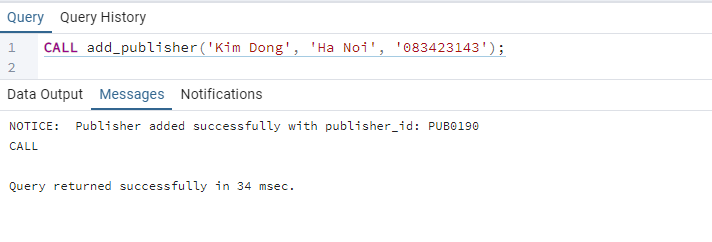
\includegraphics[width=0.95\linewidth]{Screenshot 2024-06-22 182659.png}
    \end{enumerate}
\end{enumerate}
\subsection{Tạo view}
\begin{enumerate}
    \item Tổng thành viên ở mỗi nhóm tuổi:
    \begin{enumerate}
        \item Code:
        \begin{lstlisting}
 SELECT ag.age_group_id,
    ag.age_group_name,
    count(m.account_id) AS total_members
   FROM age_groups ag
     LEFT JOIN members m ON m.date_of_birth >= (CURRENT_DATE - '1 year'::interval * ag.max_age::double precision) AND m.date_of_birth <= (CURRENT_DATE - '1 year'::interval * ag.min_age::double precision)
  GROUP BY ag.age_group_id, ag.age_group_name;
        \end{lstlisting}
        \item Kết quả:

        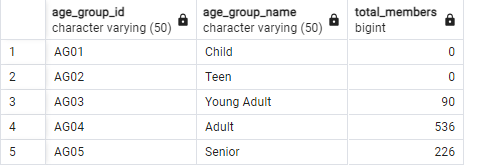
\includegraphics[width=0.95\linewidth]{Screenshot 2024-06-22 183721.png}
    \end{enumerate}
    \item Thông tin về từng đơn mượn:
    \begin{enumerate}
        \item Code:
        \begin{lstlisting}
 SELECT br.receipt_id,
    count(DISTINCT bb.book_id) AS total_books_borrowed,
    max(bb.status::text) AS status,
    sum(b.price) AS total_price,
    br.fee
   FROM borrowing_receipts br
     JOIN borrowed_books bb ON br.receipt_id::text = bb.receipt_id::text
     JOIN books b ON bb.book_id::text = b.book_id::text
  GROUP BY br.receipt_id;
        \end{lstlisting}
        \item Kết quả:

        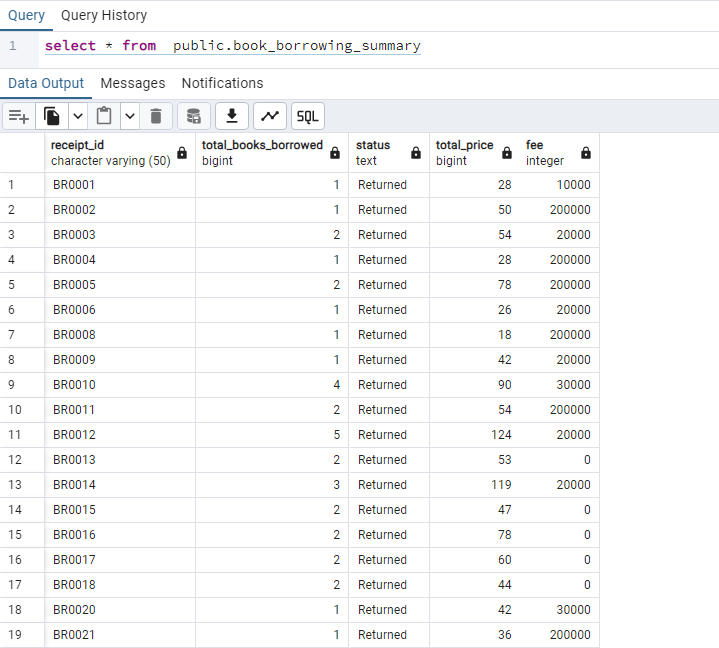
\includegraphics[width=0.95\linewidth]{Screenshot 2024-06-22 222338.png}
    \end{enumerate}
    \item Tổng sách trong kho:
    \begin{enumerate}
        \item Code:
        \begin{lstlisting}
 SELECT count(b.book_id) AS total_books,
    sum(b.quantity) AS total_quantity,
    sum(b.available) AS total_available,
    sum(
        CASE
            WHEN bb.status::text = 'Lost'::text THEN bb.quantity
            ELSE 0
        END) AS total_lost,
    sum(b.price * b.quantity) AS total_value
   FROM books b
     LEFT JOIN borrowed_books bb ON b.book_id::text = bb.book_id::text;
        \end{lstlisting}
        \item Kết quả:

        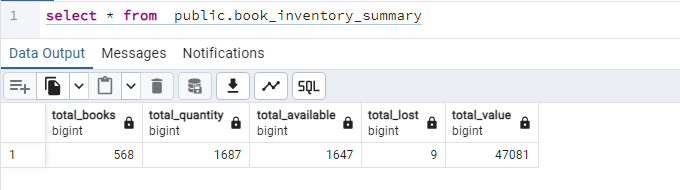
\includegraphics[width=1\linewidth]{Screenshot 2024-06-22 222825.png}
    \end{enumerate}
\end{enumerate}

\subsection{Phân quyền}
\begin{enumerate}
\item Code:
\begin{lstlisting}
-- Create roles
CREATE ROLE admin WITH LOGIN;
CREATE ROLE employee WITH LOGIN;
CREATE ROLE member WITH LOGIN;

-- Revoke all privileges on Accounts table
REVOKE ALL ON TABLE Accounts FROM PUBLIC;
REVOKE ALL ON TABLE Accounts FROM member;

-- Grant permissions to admin
GRANT ALL PRIVILEGES ON ALL TABLES IN SCHEMA public TO admin;
GRANT ALL PRIVILEGES ON ALL SEQUENCES IN SCHEMA public TO admin;
GRANT EXECUTE ON ALL FUNCTIONS IN SCHEMA public TO admin;

-- Grant permissions to employee
GRANT SELECT, INSERT, UPDATE, DELETE ON Borrowing_Receipts TO employee;
GRANT SELECT, INSERT, UPDATE, DELETE ON Books TO employee;
GRANT SELECT, INSERT, UPDATE, DELETE ON Publishers TO employee;
GRANT SELECT, INSERT, UPDATE, DELETE ON Authors TO employee;
GRANT SELECT, INSERT, UPDATE, DELETE ON Members TO employee;
GRANT SELECT, INSERT, UPDATE, DELETE ON Genres TO employee;
GRANT SELECT, INSERT, UPDATE, DELETE ON Book_Author TO employee;
GRANT SELECT, INSERT, UPDATE, DELETE ON Book_Genre TO employee;

-- Grant permissions to member
GRANT SELECT ON Books TO member;
GRANT SELECT ON Authors TO member;
GRANT SELECT ON Genres TO member;
GRANT SELECT ON Publishers TO member;
GRANT SELECT, INSERT, UPDATE ON Borrowing_Receipts TO member;
GRANT SELECT, INSERT, UPDATE ON Borrowed_Books TO member;

-- Create users and assign roles
CREATE USER admin_user WITH PASSWORD 'admin_password';
GRANT admin TO admin_user;

CREATE USER employee_user WITH PASSWORD 'employee_password';
GRANT employee TO employee_user;

CREATE USER member_user WITH PASSWORD 'member_password';
GRANT member TO member_user;

-- Grant execute permissions on specific functions to employee
GRANT EXECUTE ON FUNCTION update_book_availability_on_borrow() TO employee;
GRANT EXECUTE ON FUNCTION update_account_active_status() TO employee;
GRANT EXECUTE ON FUNCTION calculate_overdue_fees() TO employee;
GRANT EXECUTE ON FUNCTION calculate_lost_book_fees() TO employee;
GRANT EXECUTE ON FUNCTION check_quantity_limit() TO employee;
GRANT EXECUTE ON FUNCTION update_account_active_status() TO employee;
\end{lstlisting}
\item  Demo:
    \begin{itemize}
    \item Cài đặt quyền hạn là member:
        \begin{lstlisting}
 SET ROLE member; 
    \end{lstlisting}
    \item Kiểm tra quyền SELECT:
         \begin{lstlisting}
 SELECT * FROM Books; 
    \end{lstlisting}
    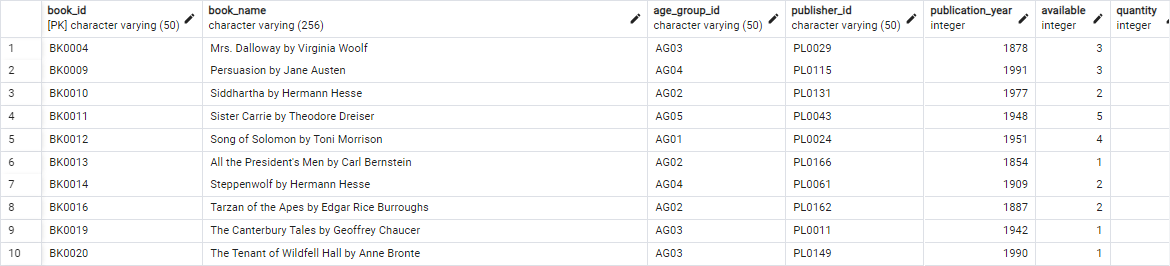
\includegraphics[width=1\linewidth]{dtb1.png}
    \item Kiểm tra quyền INSERT:
          \begin{lstlisting}
 INSERT INTO Authors (author_id, first_name, last_name, nationality)
 VALUES ('AT0307', 'John', 'Anna', 'Hungari'); 
    \end{lstlisting}
    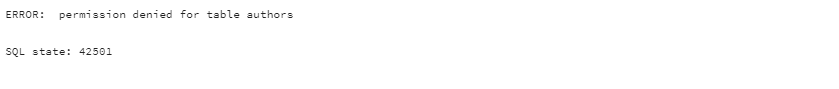
\includegraphics[width=1.1\linewidth]{dtb5.png}
    \item Kiểm tra quyền thực thi FUNCTION:
          \begin{lstlisting}
 SELECT * FROM get_author_with_most_books(); 
    \end{lstlisting}
    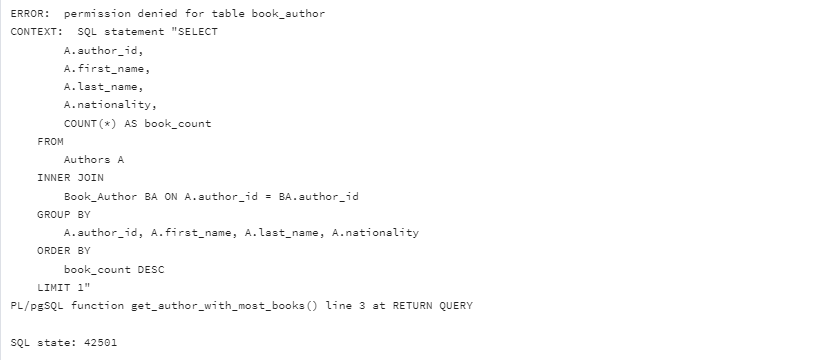
\includegraphics[width=1\linewidth]{dtb4.png}
    \end{itemize} 
\end{enumerate}    

\subsection{GUI}
\begin{enumerate}
    \item Cập nhật thông tin thành viên
\begin{itemize}
    \item Trước khi cập nhật\\
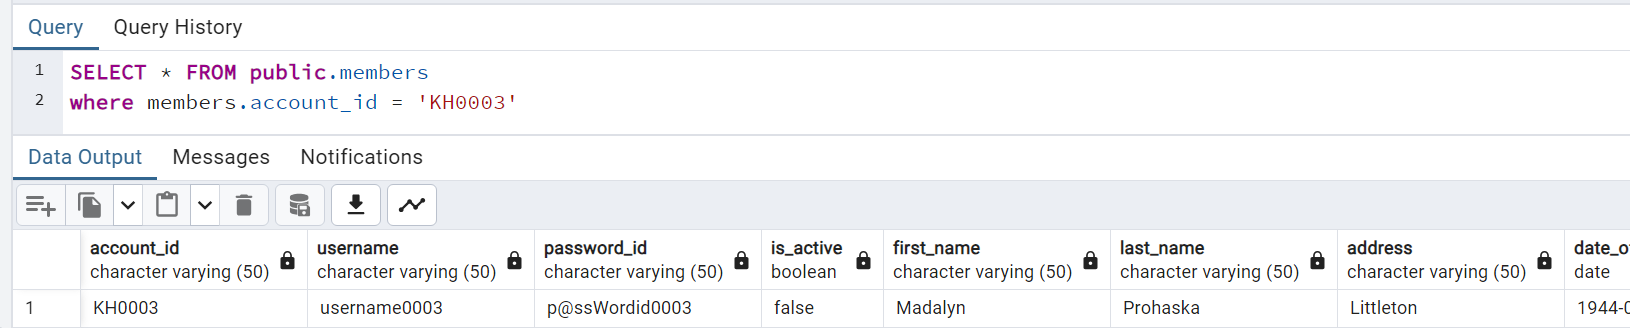
\includegraphics[width=1\linewidth]{gui1.png}
\item Nhập vào thông tin\\
\includegraphics[width=0.3\linewidth]{gui2.png}
\item Kết quả cập nhật\\
\includegraphics[width=1\linewidth]{gui3.png}
\end{itemize}

    \item Hiển thị danh sách sách theo thể loại
\begin{itemize}
    \item Kết quả\\
\includegraphics[width=1\linewidth]{gui4.png}
\end{itemize}

    \item Tổng số sách đang mượn của member
\begin{itemize}
    \item Nhập vào ID\\
\includegraphics[width=0.4\linewidth]{gui5.png}
\item Kết quả\\
\includegraphics[width=0.3\linewidth]{gui6.png}
\end{itemize}

\end{enumerate}

\section{Đánh giá hiệu năng}

\begin{table}[ht]
\centering
\begin{tabular}{|p{10cm}|p{2cm}|p{2cm}|}
    \hline
    \centering \textbf{Function and Query} & \textbf{Before optimize (ms)} & \textbf{After optimize (ms)} \\
    \hline
    get\_author\_with\_most\_books() & 9.816 & 4.732  \\
    \hline
    search\_books\_by\_keyword(key\_word) & 22.646  & 11.581  \\
    \hline
    get\_age\_group(date\_of\_birth) & 2.099  & 0.191  \\
    \hline
    find\_books\_by\_author\_name(author\_name) & 0.471  & 0.191  \\
    \hline
    get\_monthly\_borrowed\_books(year) & 1.921  & 0.980  \\
    \hline
    Procedure - Thêm sách vào thư viện & 5.610  & 2.940  \\
    \hline
    Procedure - Thêm thể loại sách & 1.31 & 1.298  \\
    \hline
    Procedure - Thêm tác giả & 2.551 & 1.556  \\
    \hline
    Đưa ra 5 đầu sách mà lứa tuổi già (senior) ưa thích nhất trong 1 năm vừa qua & 8.185  & 5.834  \\
    \hline
    Trả về top 10 đầu sách thỏa mãn có số lượng người mượn nhiều nhất trong 1 tháng kể từ thời gian gần nhất & 2.090 & 1.186 \\
    \hline
    Tính số phần trăm của các member mà tài khoản còn hoạt động trong từng nhóm tuổi & 21.394  & 12.342  \\
    \hline
    Đưa ra nhóm tuổi có số lượng người nhiều nhất & 10.681  & 8.176 \\
    \hline
\end{tabular}
\caption{So sánh hiệu suất của các hàm trước và sau khi tối ưu hóa}
\end{table}
\begin{itemize}
    \item Nhận xét: 
    
    Việc thêm  đã mang lại sự cải thiện đáng kể về hiệu suất cho hầu hết các chức năng và thủ tục trong hệ thống cơ sở dữ liệu, giúp giảm thời gian thực thi và tăng khả năng đáp ứng yêu cầu của ứng dụng.Vì khi tạo một index trên một cột trong bảng, cơ sở dữ liệu sẽ tạo ra một cấu trúc dữ liệu bổ sung (thường là cây B+ tree) để lưu trữ các giá trị của cột đó theo thứ tự nhất định.Do đó, Khi thực hiện một truy vấn SELECT với điều kiện WHERE dựa trên cột đã được tạo chỉ mục, cơ sở dữ liệu có thể nhanh chóng định vị và truy cập vào các hàng thỏa mãn điều kiện này thông qua chỉ mục. Điều này giúp giảm thời gian tìm kiếm và đọc dữ liệu, do đó tăng tốc độ truy xuất.
\end{itemize}


\section{Thu hoạch}
Sau quá trình thực hiện đồ án tạo database quản lý thư viện, chúng tôi đã thu được nhiều bài học và kinh nghiệm quý báu. Dưới đây là những kết luận và thu hoạch chính:
\begin{enumerate}
    \item Hiểu Sâu Hơn về Database Design:
    \begin{itemize}
        \item Việc thiết kế một hệ thống quản lý thư viện đòi hỏi sự hiểu biết sâu rộng về các khái niệm cơ bản trong thiết kế cơ sở dữ liệu như các kiểu dữ liệu, mối quan hệ giữa các bảng (ERD), khóa chính và khóa ngoại.
        \item Chúng tôi đã học được cách tạo ra một cấu trúc dữ liệu hợp lý, đảm bảo tính nhất quán và toàn vẹn dữ liệu.
    \end{itemize}
\item Kỹ Năng Sử Dụng SQL:
 \begin{itemize}
        \item Trong quá trình thực hiện đồ án, kỹ năng viết và tối ưu hóa các câu lệnh SQL đã được cải thiện đáng kể.
        \item Chúng tôi đã thực hành viết các truy vấn phức tạp, sử dụng các phép nối (JOIN), nhóm (GROUP BY), sắp xếp (ORDER BY) và các hàm, các trigger,..
    \end{itemize}
\item Xây Dựng và Triển Khai Database:
 \begin{itemize}
        \item Chúng tôi đã làm quen với công cụ quản lý cơ sở dữ liệu PostgreSQL.
        \item Việc triển khai cơ sở dữ liệu trên một server thực tế giúp chúng tôi hiểu rõ hơn về các vấn đề bảo mật, sao lưu và phục hồi dữ liệu.
    \end{itemize}

\item Phát Triển Kỹ Năng Giải Quyết Vấn Đề:
 \begin{itemize}
        \item Trong quá trình làm đồ án, nhiều vấn đề và lỗi phát sinh đã được giải quyết thông qua nghiên cứu và thử nghiệm.
        \item Chúng tôi đã học được cách làm việc theo nhóm, phân công nhiệm vụ và phối hợp để giải quyết các vấn đề phức tạp.
    \end{itemize}
\item Hiểu Biết về Quản Lý Thư Viện:
 \begin{itemize}
        \item Thông qua việc tìm hiểu và phân tích các yêu cầu của một hệ thống quản lý thư viện, chúng tôi đã hiểu rõ hơn về quy trình và nghiệp vụ quản lý sách, độc giả, và các giao dịch mượn/trả sách.
        \item Điều này giúp chúng tôi xây dựng được một hệ thống đáp ứng đúng nhu cầu của người sử dụng.
    \end{itemize}
\item Kinh Nghiệm Thực Tiễn:
\begin{itemize}
    \item Kinh nghiệm từ dự án này là nền tảng vững chắc để chúng tôi áp dụng vào các dự án thực tế khác trong tương lai.
 \item Chúng tôi đã có cái nhìn tổng quan về quy trình phát triển phần mềm từ giai đoạn yêu cầu, thiết kế, triển khai đến kiểm thử và bảo trì.
\end{itemize}
\end{enumerate}
\textbf{Kết Luận}:
Đồ án tạo database quản lý thư viện không chỉ giúp chúng tôi củng cố kiến thức lý thuyết mà còn rèn luyện các kỹ năng thực tiễn cần thiết cho công việc sau này. Chúng tôi tin rằng những kinh nghiệm quý báu từ đồ án này sẽ là hành trang quan trọng cho sự nghiệp lập trình và phát triển phần mềm của mỗi thành viên trong nhóm.


\end{document}